\documentclass[sigplan]{acmart}
% \documentclass{acmart}

\usepackage{graphicx}
\usepackage{hyperref}
\usepackage{float}
\usepackage{listings}
\usepackage{booktabs} % For formal tables


% Copyright
%\setcopyright{none}
%\setcopyright{acmcopyright}
%\setcopyright{acmlicensed}
\setcopyright{rightsretained}
%\setcopyright{usgov}
%\setcopyright{usgovmixed}
%\setcopyright{cagov}
%\setcopyright{cagovmixed}


% DOI
%% \acmDOI{10.475/123_4}

% ISBN
%% \acmISBN{123-4567-24-567/08/06}

%Conference
\acmConference[OSDI 2020]{SIGBOVIK}{November 2020}{Banff, Alberta, Canada}
\acmYear{2020}
\copyrightyear{2020}


%\acmBadgeL[http://ctuning.org/ae/ppopp2016.html]{ae-logo}
%\acmBadgeR[http://ctuning.org/ae/ppopp2016.html]{ae-logo}

% Document starts
\begin{document}

% Title portion. Note the short title for running heads
\title[DRAFT: Direct-style process creation on Linux]{DRAFT: Direct-style process creation on Linux}

\author{Spencer Baugh}
\affiliation{%
  \institution{Two Sigma}
  \streetaddress{100 6th Avenue}
  \city{New York City, New York}
  \country{USA}}
\email{sbaugh@twosigma.com}

\begin{abstract}
Traditional process creation interfaces,
such as fork and spawn,
are complex to use, limited in power, and difficult to abstract over.
We develop a new process creation interface for Linux
which allows a program to create a child process in an non-running state
and initialize the new process by operating on it from the outside.
This method of process creation results in more comprehensible programs, 
has better error handling,
is more efficient,
and is more amenable to abstraction.
Our implementation is immediately deployable without kernel modifications on any recent Linux kernel version.
\end{abstract}

%
% The code below should be generated by the tool at
% http://dl.acm.org/ccs.cfm
% Please copy and paste the code instead of the example below.
%
\begin{CCSXML}
<ccs2012>
   <concept>
       <concept_id>10011007.10010940.10010941.10010949.10010957</concept_id>
       <concept_desc>Software and its engineering~Process management</concept_desc>
       <concept_significance>500</concept_significance>
       </concept>
   <concept>
       <concept_id>10011007.10010940.10010941.10010949.10010950.10010951</concept_id>
       <concept_desc>Software and its engineering~Virtual memory</concept_desc>
       <concept_significance>300</concept_significance>
       </concept>
   <concept>
       <concept_id>10010147.10010169</concept_id>
       <concept_desc>Computing methodologies~Parallel computing methodologies</concept_desc>
       <concept_significance>500</concept_significance>
       </concept>
 </ccs2012>
\end{CCSXML}

\ccsdesc[500]{Software and its engineering~Process management}
\ccsdesc[300]{Software and its engineering~Virtual memory}
\ccsdesc[500]{Computing methodologies~Parallel computing methodologies}

\keywords{Process creation, Linux, fork, spawn}

\maketitle

\section{Introduction}\label{introduction}
Existing process creation interfaces can be divided into three categories:
Fork-style, spawn-style, and direct-style.

Fork-style (such as \texttt{fork}) and spawn-style (such as \texttt{posix\_spawn}) each have advantages and disadvantages.
Correct and performant usage of fork-style places significant constraints on the calling process.
Spawn-style lifts many of these constraints,
but is fundamentally limited in the kinds of processes it can create.
With both fork-style and spawn-style,
it is difficult to
branch based on results or errors encountered while initializing the new process:
fork-style requires IPC if it wishes to communicate errors back to the rest of the program,
and robust indication of errors in spawn-style requires substantial growth in the spawn interface.
Additionally, modern operating systems such as Linux have features
which are difficult or impossible to fully exploit through fork-style or spawn-style.

Direct-style is rare in general, but relatively common on academic operating systems.
\cite{keykos}\cite{sel4}\cite{exokernel}\cite{fuschia}\cite{singularity}
Direct-style involves creating a new child process in a non-running state,
and then calling individual syscalls from the parent to initialize the child.
Direct-style does not constrain the calling process,
easily branches at any step of the initialization,
and can create any kind of process supported by the underlying system.

Our contribution is an implementation of direct-style process creation for Linux,
making use of our work on the rsyscall project.
The rsyscall project develops language-specific ``process-independent'' syscall libraries for Linux,
which replace libc syscall wrappers and allow a program to perform cross-process syscalls.
rsyscall currently has best support for Python,
but can be ported to other languages;
the examples we show in this paper will be in Python,
but generalize easily to other languages.

% TODO this sounds low-content and boring.
% we should probably remove it?
% In our implementation, a parent process calls the \texttt{clone} syscall
% to create a child process which shares memory and other resources with the parent,
% and which runs no user code.
% The parent then uses \texttt{rsyscall}
% to call arbitrary syscalls in the child process to initialize it;
% for example, the parent might call \texttt{chdir} to change the child's current working directory.
% After the process is fully initialized,
% the parent can call \texttt{execve} in the child,
% causing the process to start running an arbitrary executable
% and detaching the child from the control of \texttt{rsyscall}.

Our direct-style process creation implementation uses \texttt{clone} to create a child process in an embryonic state
which can then be manipulated from user code using syscalls with \texttt{rsyscall}.
A direct-style \texttt{clone} has all the advantages of direct-style process creation
over Linux's fork-style \texttt{fork} syscall and spawn-style \texttt{posix\_spawn} libc function.
Direct-style \texttt{clone} can be used correctly and performantly from any process.
Cross-process syscalls made with rsyscall individually report errors, as normal, and can be easily branched on.
Arbitrary processes involving complex namespaces and initialization can be created
using techniques that are impractical with \texttt{fork}.
The performance cost from high-level code varies, but the underlying primitives are substantially faster.

We've implemented a variety of useful applications using direct-style process creation on Linux,
which can be expressed more concisely and more clearly than with fork-style,
which we'll showcase in brief in this paper.
Direct-style \texttt{clone} has minimal performance cost in normal situations,
and can outperform \texttt{fork} in some cases.
We've benchmarked our Python implementation of direct-style \texttt{clone}
as comparable to the Python standard library's process creation mechanism.
Finally, we have deployed direct-style process creation in production internally at Two Sigma.

Our implementation is distributed as a feature of \texttt{rsyscall},
and is immediately deployable on recent Linux kernels.
rsyscall is open source and available from \url{https://github.com/catern/rsyscall}.

This paper is organized in several sections.
In section \ref{background}, we provide background on fork-style, spawn-style, and direct-style process creation,
and consider their advantages and disadvantages in more depth.
In section \ref{overview}, we discuss the design of the API,
including our usage of \texttt{rsyscall}.
In section \ref{applications}, we show examples of usage of direct-style process creation in Python on Linux,
including use of process features which are difficult to use on Linux with \texttt{fork} or \texttt{posix\_spawn}.
In section \ref{implementation}, we explore our implementation in depth,
and discuss several difficult process-creation related details of \texttt{rsyscall}'s implementation.
In section \ref{evaluation}, we evaluate, somehow (TODO).
In section \ref{related_work},
we examine other work which also touches on the topics covered by this paper.
In section \ref{future_work},
we list several directions for future work related to direct-style process creation and to \texttt{rsyscall}.
In section \ref{conclusions}, we briefly and optimistically conclude.

\section{Background}\label{background}
Processes are a widespread feature of operating systems,
with substantial variation in characteristics between systems.
One of the areas of variation is in process creation mechanisms.

On most systems today,
the interfaces for process creation
can be divided into "fork-style" and "spawn-style".
A few systems use a third style, which we refer to as "direct-style".
\subsection{Fork-style}
By far the most well-known fork-style interface is Unix's fork.\cite{forkhist}
With a fork-style interface,
a process, called the parent process, calls \texttt{fork},
and a copy of that process is made,
called the child process,
differing only in a few attributes such as process id.
The same program continues executing in both processes,
with a different return value from fork to allow it to distinguish whether it is running in the parent or the child.
Typically, the program will case on the return value
and, if running in the child,
call various system calls to modify the state of the new process.

Fork has a number of flaws,
and much ink has been spilled detailing them.
We'll cover the most prominent briefly here,
but see Baumann 2019 \cite{forkroad} for a more detailed evaluation.

Fork, when called successfully, returns twice,
creating two different processes which execute concurrently.
This immediately makes fork difficult to integrate;
for example, errors can't be easily communicated between the two processes.
If there is an error in the initialization of the child process,
the part of the program running in the child process
needs to use some form of inter-process communication (IPC) to communicate it back to the parent process.
The child process can run arbitrary code to make decisions about its initialization,
but that code needs to use IPC if it wishes to communicate with the rest of the program,
which is still in the parent process.

Fork can have poor performance when called from processes with many memory mappings.\cite{forkroad}
Fork copies many attributes about the parent process when creating the child process,
including setting up copy-on-write memory mappings in the child process.
This becomes slower as the parent process has more memory mappings,
eventually taking a significant amount of time.
This copying is required to robustly implement fork's model,
where the same program continues executing without changes in both the parent process and child process;
the copy of the program running in the child process might access any memory at any time.

Multi-threaded programs generally cannot use fork safely.
Typical Unix fork implementations duplicate only the thread calling fork from the parent process to the child process.
In a multi-threaded program, this can cause various issues;
for example, another thread might be holding a memory allocator lock at the time of the fork,
which in the child process will never be unlocked,
causing the child process to deadlock if it tries to allocate memory.
Some thread libraries provide partial mitigations for this issue,
but it's up to user code to make use of those mitigations.\cite{pthread_atfork}
In combination with fork's poor performance in large-memory programs,
a user of fork must think carefully
about the characteristics of the process from which fork is being called.
\subsection{Spawn-style}
In a spawn-style interface,
details about the new process are provided up-front as arguments to some function
which creates the new process all at once.
The most well known spawn-style interfaces are Unix's \texttt{posix\_spawn} \cite{posix_spawn}
and Windows \texttt{CreateProcess} \cite{create_process};
the Unix shell also serves as a spawn-style process creation interface,
especially when used with Bernstein chaining.\cite{chainloading}

Spawn-style interfaces typically still transparently copy some details from the parent process;
for example, various security contexts,
and any other process attribute which is not explicitly specified in the arguments to the spawn interface.
The key difference between fork-style and spawn-style is not how much they copy,
it is how the attributes which are not copied are specified:
by mutation from code running in the new process in the case of fork-style,
or by explicit argument passing in the case of spawn-style.

Spawn-style interfaces lift the constraints on the calling process that fork-style interfaces impose.
Spawn-style interfaces don't run user code in the new process during initialization.
This means there is no need to copy memory,
so performance is good when a spawn-style interface is used from a process with many memory mappings.
Likewise, there are no inherent issues when a spawn-style interface is used from a multi-threaded program,
though operating systems which implement spawn-style interfaces on top of \texttt{fork} can still have threading bugs.

However, the arguments that can be provided to a spawn-style process creation syscall
do not cover all the possible attributes that one might want to set for the new process.
Most systems have a large number of syscalls which can mutate the state of a process during its lifetime;
for a spawn-style interface to work in all scenarios,
all those possible mutations must be reproduced in the interface.
For example, the \texttt{posix\_spawn} function provided by glibc does not support creating processes in new namespaces,
as is required for container functionality on Linux.

Spawn-style process creation
essentially creates a new domain-specific language for specifying the attributes of the process.
Fork-style allows existing system calls,
with which programmers are already familiar,
to be used to set up the new process.
Spawn-style requires some form of declarative description of the new process,
which must be learned in additional to the normal system call interface.

Spawn-style process creation also does not allow for conditional logic during the setup.
If the setup of the new process encounters an error at some point,
the only option is to return from the entire spawn call with an error.
Such errors returned from spawn-style calls
are typically much less informative
than the errors returned by the syscalls which directly mutate the process attributes.
Other forms of conditional logic are also impossible in spawn-style;
one modification to the process cannot depend on the result of some other modification.
\subsection{Direct-style}
A few academic operating systems, such as KeyKOS \cite{keykos}, seL4 \cite{sel4}
and some others \cite{exokernel} \cite{fuschia} \cite{singularity},
use another style of process creation, which we refer to as "direct-style".

In direct-style, a process is created by its parent in a non-running state,
then supplied with various resources,
and then started running once it is fully set up.
In operating systems with true direct-style process creation,
the syscalls that can mutate a process
take explicit arguments to indicate the process on which they should operate.
In this way, the same syscalls that can mutate a process while it is running,
are called by the parent process to mutate the process while it is being set up.

We refer to this as "direct-style" process creation,
because the parent creating the process operates on it directly and imperatively
rather than dispatching a distinct unit of code to perform setup from inside the context of the new process,
as in fork-style,
or building up a declarative specification of what the new process should look like ahead of time,
as in spawn-style.

Since everything happens directly from the parent process,
direct-style process creation is compatible with a variety of techniques
which are difficult with fork-style or spawn-style.
For example, a REPL could be used to interactively create the new process,
or a program might initialize several processes at once and share data between them.

Significantly,
since all operations are performed through syscalls called directly from the main program,
errors are indicated in the same way as any other syscall error.
This is unlike fork-style, which needs IPC to indicate errors,
and unlike spawn-style, which typically indicates errors at a very coarse-grained level.

Like fork-style interfaces,
direct-style interfaces can set up arbitrary attributes in the new process.
Any attribute that can be changed by a syscall
can be manipulated by a direct-style interface,
just as with fork-style interfaces.
This is unlike spawn-style interaces,
which only can change attributes that are supported by the interface.

Like spawn-style interfaces,
direct-style interfaces have no constraints on the calling process.
Also like spawn-style interface,
no user code runs in the child process, so
direct-style interfaces can be used from multi-threaded or large-memory processes without issues.

Direct-style can be more complex to use;
it is most typically used in capability-oriented operating systems,
where a great deal of resources and information must be provided explicitly to initialize the new process.
In a truly capability-oriented operating system,
nothing is copied implicitly to the new process;
everything must be explicitly specified.
This can appear more complex
when compared to process creation on Unix systems or Windows.

However, we believe that a natural port of direct-style process creation to Linux
provides an interface that is just as simple to use as fork-style or spawn-style on Linux,
without their disadvantages.
Such an interface, like fork-style and spawn-style,
would implicitly copy some attributes to the new process,
rather than being capability-oriented and requiring all attributes to be specified explicitly.
This is the kind of direct-style interface that we contribute in this paper.

\section{Overview}\label{overview}
In most operating system APIs, including the ones available on Linux,
when a program makes a syscall, it implicitly operates on the current process.
To perform direct-style process creation on Linux,
we need a Linux API where we instead explicitly specify in which process we want to make a syscall.

\texttt{rsyscall} provides this API for Linux.
The \texttt{rsyscall} project develops
language-specific, object-capability-model, low-abstraction libraries for the Linux syscall interface,
bypassing libc.

Unlike POSIX C libraries such as glibc or musl,
an rsyscall library is organized based on the object-capability model.
The capabilities to make syscalls in any given process are reified as language objects.
If the capability to make syscalls in a specific process is not passed (in some way) to a function,
then that function cannot make syscalls in that process.

Due to this design, an \texttt{rsyscall} program can make use of multiple processes at once,
by manipulating capabilities for multiple processes.
The relevant two capabilities for this paper are the initial capability to the ``local'' process,
and capabilities to child processes.
The ``local'' process is the one which hosts the runtime for the running program,
and in which a legacy libc would implicitly make syscalls;
every rsyscall program starts with the ``local'' process
and uses it to bootstrap the initial capabilities for other processes.

We use the term ``thread'' to refer to the processes under the control of rsyscall,
including the ``local'' process.
On Linux, the shared-memory ``threads'' provided by libraries such as \texttt{pthreads}
are implemented as processes,
and their lifetime and execution is completely controlled by a single program.
The same is mostly true of the controlled-process ``threads'' provided by rsyscall.
The most significant difference is that rsyscall ``threads''
do not run user code concurrently with the main program;
nevertheless rsyscall ``threads'' do provide the opportunity for concurrent execution of system calls,
and so the terminology provides useful intuition.

To perform direct-style process creation,
we use \texttt{rsyscall} to call \texttt{clone} on the ``local'' thread to create a new child thread.
We call various syscalls in the child thread to mutate it until it reaches the desired state,
at which point we can call \texttt{execve} in the child thread to start it running on its own.
After that, the process is no longer under our control, and it functions like any other child process
(hence we say ``process'' rather than ``thread'').
The child process can be monitored using normal Linux child monitoring syscalls from our main thread,
such as \texttt{waitid},
which we can also do with \texttt{rsyscall}.

\lstinputlisting[float=*,language=Python,label={basic},caption={Creating a new process, changing CWD, and execing}]
{examples/basic/direct.py}
Listing \ref{basic} shows this in action in Python.
We create a new child thread using \texttt{clone} on \verb|local_thread|,
and receive back a capability to control it.
We pass no flags to use \texttt{clone}'s defaults
(which essentially match \texttt{fork}) to create the process.
We call \texttt{chdir} in the thread to change its working directory to \texttt{/dev}.
Then we call \texttt{execve},
passing the path of the \texttt{cat} executable,
the arguments to the new executable,
and the unchanged set of environment variables.
The name of the executable is passed as the first argument,
as is typical in Unix.
Calling \texttt{execve} consumes the capability,
and later use of this child thread capability will fail with an exception.

The behavior of system calls made on a remote process through \texttt{rsyscall}
is identical to the behavior of system calls made implicitly on the current process through libc.
This is an API that systems programmers are already familiar with,
and which is already thoroughly documented through Linux system call manpages.
The novelty is constrained to the newly explicit process capabilities;
once that is understood, the rest of the API is mundane,
and the representation of these programs is obvious in any language.

The familiar and mundane nature of the API is important not just for the learning curve,
but also for expressivity.
Since the API is simply normal Linux system calls,
direct-style clone is at least as expressive as fork and syscalls;
and, in fact, as we'll see in section \ref{applications},
is significantly more expressive.
\section{Applications}\label{applications}
In this section,
we'll discuss several more advanced uses of processes,
using more sophisticated Linux features,
and accompany them with Python examples using direct-style process creation.

All of these examples use only existing Linux system calls and features.
Most are possible, though difficult to implement,
with Linux's existing \texttt{fork} system call,
and in some cases, \verb|posix_spawn|.

Direct-style makes these examples substantially easier to write;
we'll compare our implementations in this section to fork-style implementations in section \ref{evaluation}.
Furthermore, since the examples are using the Linux system call API directly,
they can be translated straightforwardly into any language with an \texttt{rsyscall} API;
Python is chosen simply for convenience.

Some of these examples showcase functionality that can be done today by specialized software and services.
Such software often allows use of one or two of these techniques, but prevents the use of others.
For example, a shell allows the creation of pipelines and container systems like Docker allow sandboxing,
but the two are difficult to combine.

By improving the process creation interface,
all these techniques can be used together, flexibly,
to more closely meet the specific needs of individual real-world applications.

For concision, we assume that we are running with sufficient permissions in these examples,
but these examples can all be run without privileges with appropriate use of \texttt{CLONE.NEWUSER}.
\subsection{Abstraction through file descriptor passing}\label{fd_abstraction}
In Linux (and Unix in general),
a program can use file descriptor inheritance
to provide file descriptors created by the parent process to child processes.
Put simply,
a new Linux child process receives copies of all file descriptors in the parent process.
When calling \texttt{execve}, these file descriptors are normally closed automatically,
but selected file descriptors can be preserved over \texttt{execve}
by disabling the \texttt{CLOEXEC} flag on individual file descriptors.
We will discuss file descriptor inheritance in more detail in section \label{fdtables},
as part of our discussion of resource management in the implementation of \texttt{rsyscall}.

Most resources in Linux are managed through file descriptors,
so this allows the parent process to pass a wide variety of resources to the child process.
An executable program can be provided a file descriptor,
which can correspond to any file in any filesystem,
or to a network connection\cite{ucspi},
or a pipe connected to another process,
or a variety of other resources,
without the process being aware of what specific resource it is accessing.
In this way, we immediately know "for free"\cite{theoremsforfree}
that the behavior of the program does not depend on the name of the file,
or the hostname to it which the socket is connected,
or the executable running in the process on the other end of the pipe,
or other abstracted-away details.

\lstinputlisting[float=*,language=Python,label={fds},caption={Passing down FDs}]
{examples/fds/direct.py}
In Listing \ref{fds},
we first open a file with read-write permission.
Then we create a child thread,
which inherits all file descriptors from its parent.
We indicate that we want to operate on the child's copy of the file descriptor with \verb|child.inherit_fd|.
\verb|inherit_fd| only updates resource-tracking bookkeeping in our program,
it makes no system calls;
the file descriptor was already copied at process creation time.
Then we disable \texttt{CLOEXEC} on the child's file descriptor,
which on Linux we can do by clearing the FD flags with \verb|fcntl(fd, F_SETFD, 0)|.
Finally, we execute some executable,
passing the file descriptor number as an argument;
when the executable starts up, that file descriptor number will already be pointing to this file descriptor.
We call the \texttt{execv} wrapper rather than \texttt{execve} as in listing \ref{basic}
so that we don't need to pass the (unmodified) environment to every exec call in these examples.
\subsection{Non-shared-memory concurrency}
Processes run concurrently,
which allows exploiting the parallelism of the underlying hardware.
Since processes don't share memory,
they can provide a less complex parallel programming environment
than shared-memory thread-based approaches.

One of the most popular parallel programming environments is the Unix shell,
which obtains its parallelism by running multiple processes connected via pipes.
The Unix shell has a relatively constrained form of parallel processing,
but it's also possible to create more complex webs of parallel processes,
where, for example, one process might take multiple inputs over multiple pipes,
or produce multiple outputs.

\lstinputlisting[float=*,language=Python,label={pipe},caption={Creating a parallel processing pipeline}]
{examples/pipe/direct.py}
In listing \ref{pipe},
we execute a few programs in parallel,
connected by pipes.
We first create two pipes,
then inherit them down to several processes using a helper function, \verb|as_argument|,
which uses \verb|inherit_fd| and \texttt{fcntl} as described in section \ref{fd_abstraction}.
We exec each program passing some file descriptors as arguments.
The whole system then runs in parallel,
as normal child processes.
\subsection{Customization without explicit support}
While, ideally, all resources would be passed by file descriptor,\cite{capsicum}
Unix has a number of resources that are global,
such as the pid space or the mount table,
and which cannot be changed on a per-process basis.

In Linux, most global resources have been made process-local
through the namespaces system.
Like other process-local resources such as the current working directory,
namespaces are typically set up at process creation time.

The most popular usage of namespaces is for large-scale container systems such as Docker;
however, this is far from the only use.
With an adaquate process creation primitive,
namespaces can be used easily on a much smaller scale.

Namespaces, like all process-local resources,
can be used to customize a program's behavior
in ways that were not anticipated by the author
by customizing the environment the process runs in.
Other system calls such as \texttt{chroot} can also be used for this.

\lstinputlisting[float=*,language=Python,label={mount},caption={Overriding absolute path using a mount namespace}]
{examples/mount/direct.py}
One classic form of customization enabled by namespaces
is overriding files at paths that were hardcoded into a program we can't change,
without changing those files for the rest of the system.
In listing \ref{mount},
we create a new child thread as normal,
but for the first time,
pass an argument to \texttt{clone}.

\verb|CLONE_NEWNS| causes clone to create the process in a new mount namespace,
which allows us to manipulate the filesystem tree in a way that only this process will see
using the \texttt{mount} system call.
We call \texttt{mount}, passing \texttt{MS.BIND}, to make the file \verb|/home/foo/custom_foo.conf|
appear at the path \verb|/etc/foo.conf|.
This is known as a bind mount.
Then we execute some executable,
which, when it opens \verb|/etc/foo.conf|, will see the contents of our \verb|custom_foo.conf|.
\subsection{Sandboxing}
At process creation time,
we can not only pass resources and customize the process's environment,
we can also deny the process access to resources that it otherwise gets by default.
This is a key part of creating a secure sandbox for potentially malicious code.

\lstinputlisting[float=*,language=Python,label={unmount},caption={Unmount all and run executable via fexec}]
{examples/unmount/direct.py}
In listing \ref{unmount}
we create a new child thread,
again in a new mount namespace using \texttt{CLONE.NEWNS}.
We open the executable that we'll later exec in this child thread,
as well as another file as in listing \ref{fds},
since we won't be able to do exec or open files normally after the next step.
Then we use \texttt{umount},
passing \texttt{MNT.DETACH} to perform a recursive unmount of the entire filesystem tree,
removing it all from the view of this process.
As in listing \ref{fds}, we unset the \texttt{CLOEXEC} flag from the database file descriptor,
so that it can be inherited across \texttt{exec};
we don't need to call \verb|inherit_fd| since, in this case, the database fd was opened directly from the child.

We then exec the file we opened earlier, using \texttt{fexec},
which allows execing a file descriptor,
and also pass the database file descriptor as an argument,
as in listing \ref{fds}.
(The underlying system call for \texttt{fexec} is \texttt{execveat};
this \texttt{fexec} is a helper function.)
Note that this executable must be statically linked,
or it wouldn't work in an empty filesystem namespace,
with no libraries to dynamically link against.

By removing the filesystem tree from the view of this process,
we can run this executable with greater confidence
that it won't be able to tamper with the rest of the system.
A sandbox which is truly robust against malicious or compromised programs requires some additional steps,
but this is a substantial start.
Such a technique can also be used when a full sandbox is not relevant,
to ease reasoning about the behavior of the program being run
and protect against bugs.

Even if the process needs additional resources,
those can be explicitly passed down through file descriptor passing,
as we do here with the database file descriptor.
This is the essence of capability-based security,
which Linux can increasingly closely approximate.
\subsection{Nested clone and pid namespaces}
Process-local resources can also be used to control the lifetime of resources used by that process.
Many Linux resources are not automatically cleaned up on process exit;
a poorly coded program may allocate global resources
and not ensure that they are cleaned up,
leaving behind unused garbage on the system.

One resource which is not automatically cleaned up is processes themselves;
if we run a program which itself spawns subprocesses,
those subprocesses may unintentionally leak,
and be left running on the system even after the program itself has stopped.

We can use a pid namespace to solve this issue.
The lifetime of all processes in a pid namespace is tied to the first process created in it,
the init process.
When the init process dies,
all other processes in the pid namespace are destroyed.

\lstinputlisting[float=*,language=Python,label={pidns},caption={Nested clone and pid namespace}]
{examples/pidns/direct.py}
In listing \ref{pidns},
we create a child process which we call \texttt{init},
passing \verb|CLONE_NEWPID| to create it in a new pid namespace.

To create another process in the pid namespace,
we clone again, this time from \texttt{init}.
This is the first example in which we've cloned from one of our child threads;
as normal, this produces a new process, a grandchild,
which can be used exactly like a direct child thread.
We exec in the grandchild,
and we can monitor the grandchild process from \texttt{init},
just as we would monitor \texttt{init} from its parent process.

\texttt{init} in a pid namespace has some special powers and responsibilities.
We can handle these responsibilities ourselves directly from our program,
or we can continue on by execing an init daemon in \texttt{init} to handle it for us.

In either case, when \texttt{init} dies,
the pid namespace will be destroyed,
and \texttt{grandchild} will be cleaned up.
\subsection{Shared file descriptor tables}\label{shared_fd_table}
A library can create a child process to perform a useful service.
This can sometimes be done more easily when the child process shares file descriptors with the parent.

\lstinputlisting[float=*,language=Python,label={fuse},caption={Shared file descriptor tables}]
{examples/fuse/direct.py}
In listing \ref{fuse},
we first create a child process, \verb|ns_child|, in a new mount namespace with \verb|CLONE_NEWNS|,
and for the first time, also pass \verb|CLONE_FILES|,
which causes the file descriptor table to be shared between the parent process and the child process.
We create a grandchild off of \verb|ns_child|,
and use it to exec a FUSE filesystem,
which will appear only in the mount namespace of \verb|ns_child| and its descendents.
Then we can open FUSE files in \verb|ns_child|
and use those files in the parent process,
through the shared file descriptor table.

File descriptor passing over a Unix domain socket
can allow similar behavior without sharing the file descriptor table,
but is substantially more complex for the user.
Nevertheless, for fork-style and spawn-style process creation,
file descriptor passing over a Unix domain socket
is the only option to do something like this.
\section{Implementation}\label{implementation}
\subsection{Basics about rsyscall}
In this section, we'll give a brief overview of the implementation of rsyscall,
and then focus on implementation issues specific to process creation.

rsyscall can be conceptually divided in two parts:
the basic cross-process syscall primitive,
and a language-specific library built on top.
The Python language-specific library has already been demonstrated above.
Such libraries only need to be able to call syscalls and explicitly specify a process in some way;
they are, for the most part, agnostic to how the cross-process syscall is implemented.

On Linux \verb|x86_64|, a syscall is specified by a syscall number plus six register-sized arguments;
a syscall returns one register-sized value.
rsyscall's default implementation of cross-process syscalls sends those seven integers over a pipe,
and waits for a response on another pipe.
Processes are created running an infinite loop which, at each iteration,
reads a syscall request off the pipe,
performs that syscall,
and writes the return value back over the return pipe.
In this way, a cross-process syscall works much like a very primitive remote procedure call.

We use pipes (or other file descriptors) for transport of data rather than a shared memory segment
to support straightforward integration with event loops.

ptrace provides an alternative means to perform arbitrary actions on other processes,
including system calls.
However, among other issues, it has the unavoidable substantial disadvantage of not permitting multiple ptracers.
A ptrace-based implementation would prevent using strace or gdb on rsyscall-controlled processes,
which is an unacceptable limitation for a general-purpose utility.

Many syscalls either take or return pointers to memory,
and require the caller to read or write that memory to provide arguments or receive results.
Therefore, an rsyscall library needs a way to access memory in the target process.

The most simple way to access memory is for the main thread to be in the same address space as the target process.
This is the case most of the time; we pass \texttt{CLONE.VM} by default in the Python wrapper.
However, the target process may be in another address.
For example, if the target process is at a different privilege level,
it must be in a different address space,
as sharing an address space with a process at a different privilege level is unsafe.

We implement access to the memory of processes in different address spaces through another set of pipes,
by explicitly copying memory into and out of those pipes using the \texttt{read} and \texttt{write} system calls.
When we wish to read \texttt{N} bytes of memory at address \texttt{A} in the target process,
we first perform a \verb|write(memory_pipe, A, N)| in the target process,
and then read that data off the other end of the pipe in the parent process.
When we wish to write \texttt{N} bytes of data at address \texttt{A} in the target process,
we first write that data to the pipe in the parent process,
then perform a \verb|read(memory_pipe, A, N)| in the target process to copy that data from the pipe into memory.

The \verb|process_vm_readv| and \verb|process_vm_writev| system calls
allow the caller to read and write memory from the virtual address space of other processes.
However, they require that the caller have specific credentials relative to the process being accessed,
which may not always be the case.
Additionally, these system calls are disabled if ptrace is disabled system-wide,
which is a niche but possible system configuration.
To ensure that rsyscall can be used for arbitrary purposes and on arbitrary systems, we avoided these calls.
\subsection{\texttt{clone}}\label{clone}
Now that we've established the basic implementation details of rsyscall,
we'll consider specific issues related to process creation and initialization.

There are three Linux system calls which create processes:
\texttt{fork}, \texttt{vfork} and \texttt{clone}.
\texttt{vfork} suspends execution of the parent process
while waiting for the child process to exit or call \texttt{execve},
which is immediately unsuitable for direct-style process creation.
\texttt{clone} provides a superset of the functionality of \texttt{fork},
so we focused our attention on \texttt{clone}.

\texttt{clone} (along with \texttt{fork}) creates a new process
which immediately starts executing at the next instruction after the syscall instruction,
in parallel with the parent process,
with its registers in generally the same state as the parent process.
\footnote{Note that =glibc= defines a wrapper for the clone syscall;
we are talking about the raw kernel syscall.}
In the style of Plan 9's \texttt{fork} syscall\cite{rfork}, which inspired \texttt{clone},
\texttt{clone} takes a mask of flags which determines whether several attributes of the new process
are either shared with, or copied from, the parent process.

\texttt{clone} only lets us change the stack for the new process;
the new process begins executing, after \texttt{clone}, at the same instruction as the parent process.
We would like to be able to set arbitrary registers for the new process,
so that we can control where it begins executing and the stack it executes on.

Fortunately, changing the stack is sufficient.
We ensure that the next instruction executed after any syscall is a \texttt{RET}.
Since we control the state of the stack in the new process after a \texttt{clone} syscall,
the \texttt{RET} will jump to a code address that we control.
We can then supply additional arguments to this code
by putting them on the stack.

We typically cause the new process to jump to a trampoline provided by the rsyscall library
which sets all registers to values found on the stack
and then jumps to another address.
\footnote{This is also a generally useful utility for hackers performing return-oriented-programming attacks;
but similar functionality exists in any standards-compliant C library,
so there is no increase in attack surface.}
With this trampoline,
we can provide a helper Python function that,
when given a function pointer following C calling conventions, and some arguments,
will prepare a stack for a call to clone such that the new process will call that function with those arguments.

With our new ability to call arbitrary C-compatible functions,
we can now call \texttt{clone} so that it launches a process running our infinite syscall loop,
which is implented in freestanding C and, as described in the previous section,
uses two pipes passed as arguments to receive syscall requests and respond with syscall results.

After using \texttt{clone} to create a new process running our syscall loop,
most system calls can be called as normal.
The new process can be modified freely through \texttt{chdir}, \texttt{dup2}, and other system calls.
Out of system calls related to process creation,
only \texttt{execve} and \texttt{unshare} need substantial further attention.
\subsection{\texttt{exec}}
\texttt{execve} is unusual and requires careful design,
because when it is successful, it does not return.
Therefore we need a way to determine if \texttt{execve} is successful;
naively waiting for a response to the syscall request will leave us waiting forever.

There is a traditional technique to detect a successful \texttt{execve} using a pipe.
We create a pipe before forking,
ensure both ends are marked \verb|O_CLOEXEC|,
perform the fork,
call \texttt{execve} in the child,
close the write end of the pipe,
and wait for EOF on the read end.
If the child process has neither successfully called \texttt{execve}, nor exited for some other reason,
then the write end of the pipe will still be open in the child process's fd table,
and the read end of the pipe will not return EOF.
But once the child process calls \texttt{execve} successfully,
\verb|O_CLOEXEC| will cause the write end of the pipe to be closed,
and the read end of the pipe will return EOF.

This trick works well with \texttt{fork};
but it's not general enough to work with \texttt{clone}.
Child processes can be created with the \verb|CLONE_FILES| flag passed to \texttt{clone},
which causes the parent process and child process to share a single fd table;
we showed an example of this in section \ref{shared_fd_table}.
This means that when the parent process closes the write end of the pipe,
it will also be closed in the child process,
and the read end of the pipe will immediately return EOF,
regardless of whether the child has called \texttt{execve} or exited.

Fortunately, there is an alternative solution, which does work with \verb|CLONE_FILES|.
The \texttt{ctid} argument to \texttt{clone} specifies a memory address which,
when the \verb|CLONE_CHILD_CLEARTID| flag is set,
the kernel sets to zero when the child exits or execs,
and then, crucially, performs a futex wakeup on.
More specifically,
the kernel clears and does a futex wakeup on \texttt{ctid} when the child process leaves its current address space;
this precisely coincides with exiting or execing,
since those are the only way to change address space in Linux as of this writing.

A futex is a Linux-specific feature,
which is generally used for the implementation of userspace shared-memory synchronization constructs,
such as mutexes and condition variables.
The relevant detail for us here is that we can wait on an address
until a futex wakeup is performed on that address;
that means we can wait on \texttt{ctid} until the futex wakeup is performed,
and in this way get notified of the child process calling \texttt{execve}.

Unfortunately, futexes in current Linux integrate poorly:
There is no way for a single process to wait for more than one futex at a time,
and no way to monitor a futex with file-descriptor-monitoring syscalls such as \texttt{poll}.
The best we can do is create a dedicated child process for each futex we want to wait on,
and have this child process exit when the futex has a wakeup.
Monitoring child processes can be straightforwardly integrated into an event loop.

While slightly complex to implement, this solution works well.
We provide \texttt{ctid} whenever we call \texttt{clone},
and set up a process to wait on that futex.
Then, when we call any syscall,
we wait for either the syscall to return an error or the futex process to exit,
whichever comes first.
Either will normally indicate that the syscall fails,
but if the futex process exits,
without the child process itself exiting,
then we can catch that in \texttt{execve} and know that the child has successfully called \texttt{execve}.

If the futex process and child process both exit,
it's ambiguous whether the child process successfully called \texttt{execve};
this ambiguity is unfortunate, but it is also present in the pipe-based approach.
This is, we believe, the best solution currently available.

We would prefer for Linux to natively provide functionality to wait for a child's \texttt{execve}.
Some other Unix-like systems provide this;
kqueue, on FreeBSD, allows waiting for exec in arbitrary processes through kqueue's \verb|EVFILT_PROC|.

One approach for Linux would be to add a new \texttt{clone} flag to
opt-in to receiving \texttt{WEXECED} events through \texttt{waitid};
note that a \texttt{waitid} flag alone is not sufficient,
since it's necessary to receive \texttt{SIGCHLD} signals for the \texttt{WEXECED} event if waiting for it from an event loop.

Alternatively, some way to wait for futex wakeups through a file descriptor could be added,
so we can use file-descriptor-monitoring syscalls to wait for the \texttt{ctid} futex;
such a feature used to exist in the form of \verb|FUTEX_FD|,
but was removed from Linux long ago due to race conditions in its design.
\subsection{Managing file descriptor tables}\label{fdtables}
As demonstrated in section \ref{shared_fd_table},
the \verb|CLONE_FILES| flag can be passed to \texttt{clone},
causing the file descriptor table to be shared between the parent process and child process.
The same file descriptors are open in both processes at the same numbers,
and if new file descriptors are opened in either process,
they are also visible in the other process.
This is simple to model, and convenient for many purposes.
The file descriptor table is unshared once the child calls \texttt{execve}.

If \verb|CLONE_FILES| is not passed to \texttt{clone},
then \texttt{clone} has the same behavior as \texttt{fork}:
The new process has a new file descriptor table,
containing copies of all the file descriptors existing in the parent at the time of the system call.
This is known as file descriptor inheritance.

This same behavior can also be triggered after process creation by calling \verb|unshare(CLONE_FILES)| or \texttt{execve}.
If \verb|unshare(CLONE_FILES)|
is called in a process currently sharing its file descriptor table with another process,
then after the call that process will have a new, private file descriptor table,
again with a copy of all the file descriptors existing at the time of the system call.

If \texttt{execve} is called,
the treatment of the file descriptor table is the same as \verb|unshare(CLONE_FILES)|,
except that file descriptors with the \texttt{CLOEXEC} flag set on them
are not copied into the newly created file descriptor table.
In standard Unix practice, \texttt{CLOEXEC} is set habitually by users on all file descriptors;
we'll discuss the semantics of \texttt{CLOEXEC} more in section \ref{cloexec}.
\subsubsection{Tracking file descriptors through handles}
After a system call has copied all the file descriptors in the old table into the new table,
we need to decide which file descriptors we want to keep open in the new table,
and which file descriptors should be closed.

This is a question of resource management.
In a language with manual resource management,
such as C,
this would be delegated to the user,
and the responsibilities of the \texttt{rsyscall} library would end there.
Manual resource management in C has led to many bugs,
many of which with significant security implications.

Python, however, is a garbage collected language,
and therefore we determine which file descriptors should stay open through garbage collection:
if a certain file descriptor is in use by the program,
through a certain process,
that file descriptor should stay open in that process's file descriptor table.

To achieve this, file descriptors are used through garbage-collected handles;
each handle is associated with a process and contains a specific file descriptor number.
For a handle to remain valid,
that file descriptor number must continue to refer to an open file descriptor in that process.
We determine which handles are live (in use by the program)
by recourse to the native Python garbage collection system.
We keep open exactly what file descriptors are necessary to keep the live handles valid.

When a process changes file descriptor table through \verb|unshare(CLONE_FILES)|,
we need to make sure all the live file descriptor handles associated with that process continue to be valid.
This is straightforward:
we enumerate all the handles associated with the process,
and don't close the file descriptors that those handles refer to.

Likewise, if a process changes file descriptor table through \texttt{execve}
in a way that allows the program to keep control of the process,
we make sure to keep all the file descriptors with live handles open.
This requires careful management of \texttt{CLOEXEC}.

When a process is newly created,
no file descriptor handles yet exist;
New handles can be created by opening files in the process,
or by using the \verb|inherit_fd| function to create handles for inherited file descriptors.
\verb|inherit_fd| takes a file descriptor handle associated with the parent process,
and, if that file descriptor was open at the time the child process was created,
creates a new handle associated with the child process
for the child process's copy of that file descriptor.
Once the inherited file descriptors are closed as described in section \ref{cloexec},
\verb|inherit_fd| can't be used again until the process next changes file descriptor table.
\subsubsection{Closing file descriptors after inheritance}\label{cloexec}
After creating a new file descriptor table,
and establishing which file descriptors should be kept open,
we must promptly close other file descriptors.
Leaving unwanted file descriptors open in the new table is a form of resource leakage.
It can also cause erroneous behavior.
For example, it's a common practice to close the write end of a pipe
and expect an EOF on the read end;
if the write end is copied into the new file descriptor table before being closed,
and the write end is never closed in the new table,
the read end will never get an EOF.

However, we can't simply close all other file descriptors,
because we must preserve the semantics of implicit file descriptor inheritance.
The possibility of implicit inheritance of file descriptors is a traditional Unix feature,
which is useful in a wide variety of situations,
in much the same way as environment variables, which are also implicitly inherited.
As with environment variables,
implicitly inherited file descriptors allow a resource to be passed down a process hierarchy
without intervening programs being aware;
this is a form of dynamic scope, which, though notorious, is often useful.

Fortunately, file descriptors which should be implicitly inherited are marked:
they have \texttt{CLOEXEC} turned off.
For implicit inheritance to function, \texttt{CLOEXEC} must not be set;
otherwise, the file descriptor will be closed, rather than inherited,
the next time the process calls \texttt{execve}.
And since \texttt{execve} can be called at any time in a general purpose program,
any library that does not want its file descriptors to be inherited across \texttt{execve}
must keep \texttt{CLOEXEC} turned on at all times.
So, at any time, we know that the file descriptors with \texttt{CLOEXEC} off
are exactly the file descriptors which should be implicitly inherited.

Therefore, we simply need to close all file descriptors that have \texttt{CLOEXEC} set,
and which are not referenced by a live file descriptor handle;
we refer to this operation as \verb|close_cloexec|.

For \verb|unshare(CLONE_FILES)|, we perform \verb|close_cloexec| automatically in userspace.
For \texttt{clone}, we perform \verb|close_cloexec| closing operation only on user request,
so that the user can control when \verb|inherit_fd| stops working.
Even if the user never requests that unused file descriptors be closed,
as long as they call \texttt{execve}, the table will be cleaned at that point.
In both of these cases,
it would be beneficial for efficiency to delegate \verb|close_cloexec|
to a new system call which takes a list of file descriptors
and closes all \texttt{CLOEXEC} file descriptors except for those on the list.

For \texttt{execve}, this oepration is, in some sense, done automatically for us by the kernel;
except we don't get the chance to preserve live file descriptors handles,
without first unsetting \texttt{CLOEXEC} on them.
Again an extension to the kernel would be useful:
A new argument to \texttt{execve} which allows specifying a list of file descriptor numbers to inherit
despite the \texttt{CLOEXEC} flag.
This would allow programs to avoid the pattern
of unsetting \texttt{CLOEXEC}, calling \texttt{execve}, and then immediately re-setting \texttt{CLOEXEC},
just to inherit a file descriptor across a single exec.
This might seem minor,
but unsetting \texttt{CLOEXEC} before \texttt{execve} is not possible
when the process calling \texttt{execve} has a shared file descriptor table,
because some other process might call \texttt{execve} as well,
and erroneously inherit the file descriptor.
\section{Evaluation \textbf{TODO}}\label{evaluation}

We quantitatively answer the following questions:
\begin{itemize}
\item
  Does direct-style process creation on Linux allow for simpler programs than the alternatives?
  We implement and compare similar functionality using both direct-style and fork-style in \ref{ease}.
\item
  Does a clone-based implementation avoid the well-known performance overheads of fork?
  We evaluate clone against fork on several microbenchmarks in \ref{microbench}.
\item
  Does a high-level Python direct-style process creation interface
  have acceptable performance relative to the Python standard library's spawn-style interface?
  We benchmark direct-style process creation against spawn-style in \ref{subprocess_bench}.
% TODO have an item about use at TS? hm.
% could be qualitative
\end{itemize}
\subsection{Ease of programming with direct-style}\label{ease}
\begin{table}
\begin{tabular}{rrrr}
\hline
Name & Listing & Direct-style & Fork-style \\
\hline
basic & \ref{lst:basic} & 3 & 14 \\
fds & \ref{lst:fds} & 6 & 16 \\
pipe & \ref{lst:pipe} & 17 & 49 \\
mount & \ref{lst:mount} & 4 & 15 \\
unmount & \ref{lst:unmount} & 7 & 18 \\
pidns & \ref{lst:pidns} & 3 & 23 \\
fuse & \ref{lst:fuse} & 6 & 27 \\
\hline
\end{tabular}

\caption{Line counts with direct-style vs fork-style}
\label{tab:ease}
\end{table}
We implement a variety of simple but powerful techniques with processes
using both direct-style and fork.
Our results are summarized in table \ref{tab:ease}.
Direct-style consistently takes under half the lines the express the same thing.
\lstinputlisting[float=*,language=Python,label={basic_fork},caption={Fork-style: Creating a new process, changing CWD, and execing}]
{examples/basic/fork.py}
An example of one of the fork-style implementations is in listing \ref{basic_fork}.
It corresponds to the direct-style example in listing \ref{basic}.

In our fork-style implementations,
we assume a great deal of infrastructure is available to make fork-style simpler.
We assume the existence of a robust IPC system,
with an already-defined protocol which can cover all errors from all system calls.
Despite this, fork-style implementations are still significantly more verbose than direct-style.
\subsection{Clone versus fork}\label{microbench}
\begin{figure}[h!]
\centering
 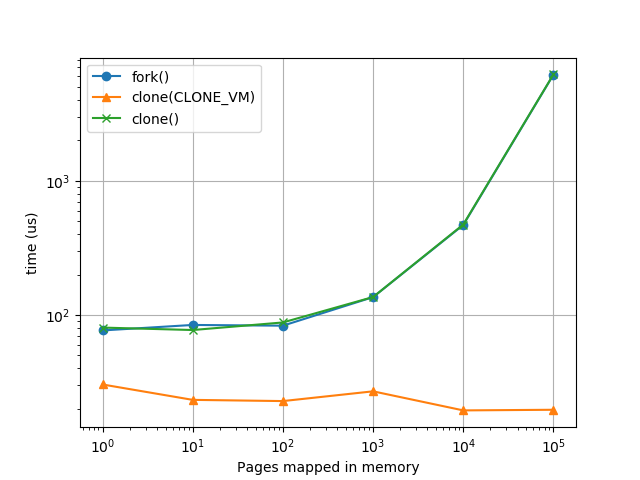
\includegraphics[width=0.5\textwidth]{microbench}
 \caption{fork and clone performance under varying memory usage}
 \label{fig:microbench}
\end{figure}

We run a benchmark which times how long process creation takes
with \texttt{fork}, \texttt{clone}, and \verb|clone(CLONE_VM)|
with varying amounts of anonymous memory mapped in the parent process
before running the benchmark.
\texttt{clone} without \verb|CLONE_VM| functions identically to fork.
The results are in figure \ref{fig:microbench}.
Without \verb|CLONE_VM|,
process creation time is linear in the amount of memory mapped in the parent process.
At the upper end of our benchmark, with 4 GB of memory mapped ($10^6$ pages),
\texttt{fork} takes an average of 42.6 milliseconds to create a process,
while \verb|clone(CLONE_VM)| stays flat at 21.1 microseconds.

This is because \texttt{fork}, and \texttt{clone} without \verb|CLONE_VM|,
must set up memory mappings in the child process for all the memory mapped in the parent process.
\verb|clone(CLONE_VM)| does not have to do this bookkeeping,
so its process creation time is constant in the amount of memory used in the parent process.

\subsection{High-level direct-style versus spawn-style}\label{subprocess_bench}
\begin{figure}[h!]
\centering
 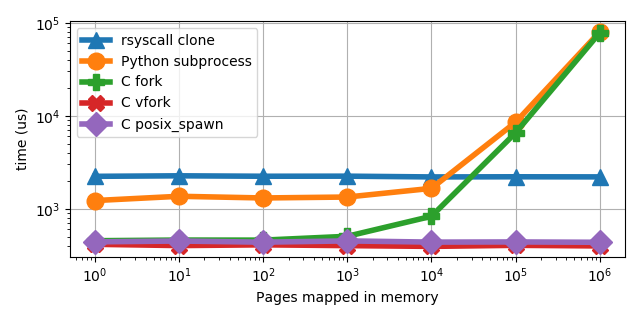
\includegraphics[width=0.5\textwidth]{subprocess_bench}
 \caption{Python subprocess and direct-style clone performance under varying memory usage}
 \label{fig:subprocess_bench}
\end{figure}

We benchmark Python's \texttt{subprocess.run} against direct-style \texttt{clone} with \texttt{rsyscall}
with varying memory usage, as in section \ref{microbench}.
The results are in Figure \ref{fig:subprocess_bench}.
TODO generate again to get the higher end where it crosses over.
\section{Related work}\label{related_work}
% TODO all this is just slapped onto the page without much thought, needs revising
\subsection{Direct-style process creation}
As we discuss in section \ref{background},
many academic operating systems have direct-style process creation.
We are not aware of any previous instances of direct-style process creation in a Unix-like environment.

The closest related work known to us
is efforts to build Unix compatibility environments, including fork-style process creation,
on academic operating systems which natively use direct-style process creation.\cite{exokernel}
Such compatibility environments could theoretically be bypassed to perform direct-style process creation
using the underlying primitives,
but regular Unix system calls could not be used to create new Unix processes in a direct-style way
in such an environment.
\subsection{Remote system calls}
There are many Unix-based systems which do something called "remote system calls".
Most such systems do not allow a single program to manipulate multiple processes.
Those systems that do allow manipulating multiple processes
are generally oriented towards debugging and introspection,
and are unsuitable for a general purpose system.

Many systems use system call forwarding to implement migration in a computing cluster.
HTCondor\cite{condor} and Popcorn\cite{popcorn} are two examples.
In both systems, processes can be live-migrated between hosts;
when this occurs, the system will automatically forward IO-related system calls
back to the original host.

Some systems intercept system calls and forward them to another process to be implemented
as part of a virtualization system.
gvisor\cite{gvisor} and ViewOS\cite{viewos} are two examples.
In both systems,
system calls made in one process are intercepted,
and serviced by another process.
Also relevant is seccomp system call interception,
which can be used to intercept system calls and emulate them in another process.

Some systems forward system calls elsewhere for asynchronous execution.
FlexSC\cite{flexsc} is one example.
System calls were forwarded to dedicated system call execution threads.
The recently added Linux feature \verb|io_uring| is, in some sense, another example;
it supports sending a subset of system calls to the kernel,
which executes them asynchronously,
rather than blocking the thread.

Some systems call system calls in other processes for debugging or introspection purposes.
strace, gdb, and CRIU\cite{criu} are examples of this.
These systems typically uses ptrace,
which is capable of operating on multiple processes at once.
Unfortunately, as discussed in section \ref{implementation},
ptrace is unsuitable as a mechanism for a general purpose system since it is not re-entrant;
a process which is already being ptraced cannot be ptraced again,
so using ptrace as a cross-process system call mechanism would disallow use of strace or debuggers.
\subsection{Process capabilities}
We mentioned the concept of process capabilities while discussing the design of rsyscall in section \ref{overview}.
The Capsicum system provides something called process descriptors\cite{capsicum},
which is a file descriptor handle for a process.
A similar feature has been recently added to Linux in the form of the pidfd API\cite{pidfd}.
These notions of process capability are quite limited, however;
pidfds and process descriptors only allow sending signals to a process or waiting for its death,
rather than exercising full control over the process.
\subsection{Capability-secure libc replacements}
The Capsicum system provides a set of system calls
which can be used to provide a capability-secure sandbox.\cite{capsicum}
Latter efforts\cite{oblivious}, including CloudABI\cite{cloudabi} and WASI\cite{wasi},
are focused primarily on backwards compatibility with the existing POSIX environment, and ease of porting existing code.
Programs ported to the capability-secure environment
are typically launched with an accompanying spawn-style wrapper.
This means that capability-secure processes are created primarily by an API
that is distinct from the capability-secure syscall API they have access to,
which makes it harder for a capability-secure process to spawn further capability-secure processes of its own.
Direct-style process creation could make it easier to create capability-secure processes 
from the capability-secure syscall API,
and reduce the need for a separate spawn-style wrapper.

Also related is the PLASH, ``Principle of Least Authority Shell''\cite{plash}.
PLASH provides a spawn-style API (in the form of a shell)
to launch processes in a capability-secure environment.
PLASH, like all spawn-style APIs, abstracts over the native Linux environment,
and is therefore limited in what kind of processes it can create.
\section{Future work}\label{future_work}
\subsection{Other applications of rsyscall}
Most avenues of future work focus on rsyscall.
rsyscall was not developed solely for the purpose of this paper,
and it has many uses unrelated to direct-style process creation,
such as asynchronous system calls, exceptionless system calls\cite{flexsc}, cross-host operations, among others.
We are actively exploring such applications,
as well as broadening rsyscall's language support.
\subsection{Kernel support}
rsyscall's cross-process syscalls can be performed entirely in userspace,
which has substantial benefits for deployability.
Nevertheless, direct kernel support for creating a stub process and performing syscalls in the context of that process
may provide efficiency benefits, as well as reducing userspace-visible complexity.

Several other aspects of our implementation would be improved by kernel support.
We discussed these in the implementation section;
in brief, we would most benefit from kernel support for
detecting when a child process finishes =execve=,
closing all =CLOEXEC= file descriptors except for an explicitly specified list,
and explicitly specifying a list of =CLOEXEC= file descriptors to inherit over =excve=.
Implementing these features in the kernel in a generally useful way, and upstreaming them,
is an important direction for our future work.
\subsection{Portability to other Unix systems}
Other non-Linux systems
could adopt the techniques of this paper
to provide direct-style process creation.
Currently, our focus is on Linux,
but others may wish to explore porting these techniques to other operating systems.
\subsection{Large scale open source usage}
We have made use of the techniques described in this paper
in proprietary software at Two Sigma.
While this gives us personally greater confidence in these techniques,
it would be better to use them in a publicly available, open source system.
Either porting an existing system to use these techniques,
or using these techniques to create a substantial new system from scratch,
would provide a meaningful demonstration of the viability of these techniques.
% \subsection{file descriptor lifetime management}
% % TODO this is hard to explain, probably best to drop this
% Keeping file descriptors open if and only if there is a specific process using that file descriptor
% is not the only possibility.
% Keep in mind that "a process using the file descriptor" is a slight abuse of terminology;
% processes don't use file descriptors, programs do, and in our system there is only one program.
% To reflect this, we could instead more directly use file descriptors in a process-agnostic way;
% this would support the creation of objects
% which work transparently across multiple processes which share a file descriptor table.
% Such objects would automatically use the relevant process to perform the syscalls for any specific operation.
% A process-centric view of file descriptors instead forces each object to be associated with one process.
% Nevertheless, we found that the process-centric perspective better matches the existing intuitions of users,
% especially those with prior experience in programming with processes.
% We hope that future systems for multi-process programming
% might explore an object-centric approach for managing resources.
\section{Conclusions}\label{conclusions}
Direct-style process creation is much less known and much less used than fork-style and spawn-style.
We have implemented direct-style process creation for Linux.
Our implementation is immediately deployable on today's Linux systems.
We have discussed various applications of processes,
and demonstrated the use of Linux direct-style process creation
to implement them.
We hope that this work will help encourage more use of the process abstraction,
which, though widespread,
is still not used to its full potential.

\bibliographystyle{ACM-Reference-Format}
\bibliography{bibliography}
\end{document}
